% Autor: Elias Welt
\section{Admin Panel (AdminPanel.jsx)}

Das \texttt{AdminPanel.jsx} ist das Kontrollzentrum für Systemadministratoren und demonstriert fortgeschrittene Patterns wie zweistufige Zugriffssicherung und kaskadierende Datenabfragen. Der Zugriff auf diese Route wird auf zwei Ebenen geschützt:

\begin{figure}[h]
    \centering
    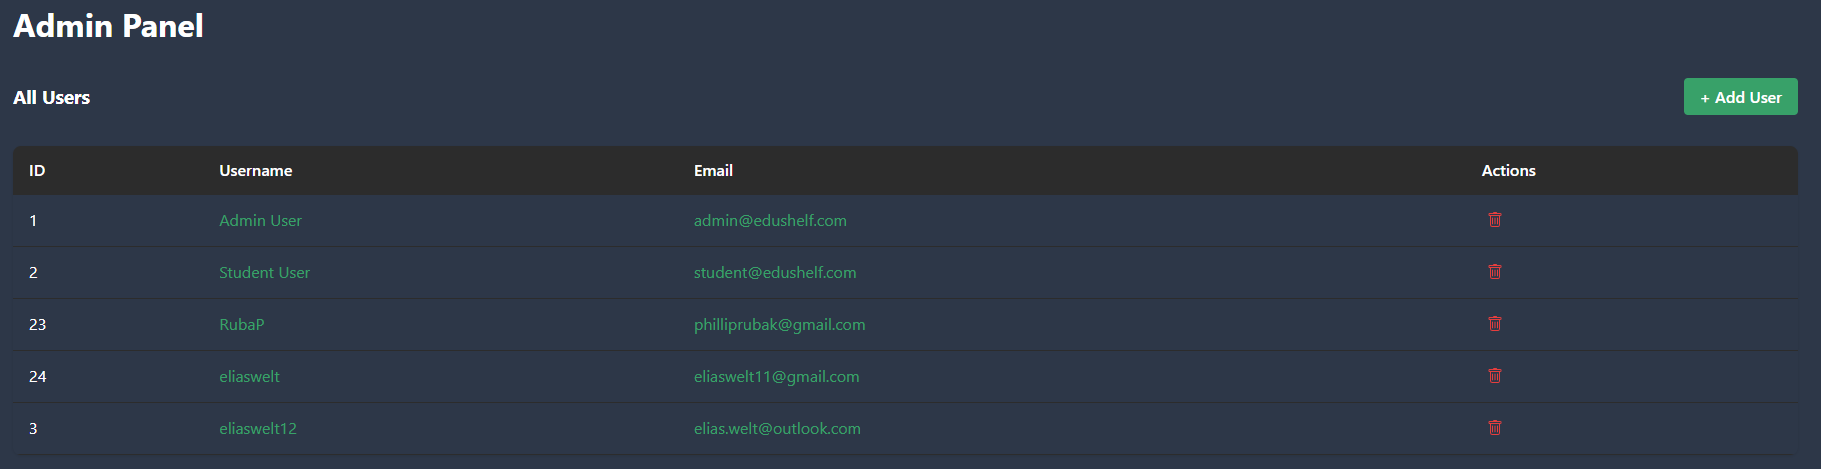
\includegraphics[width=0.92\textwidth]{img/admin-panel-dark-mode}
    \caption{Admin-Panel von EduShelf im Dark-Mode}
    \label{fig:admin-panel}
\end{figure}


\subsection{Zweistufige Zugriffssicherung (RBAC)}

\begin{itemize}
    \item \textbf{1. Client-Side Routing}: In \texttt{App.jsx} wird geprüft, ob das Benutzerobjekt die Rolle \textit{Admin} enthält. Falls nicht, wird der Nutzer sofort umgeleitet.
    \item \textbf{2. Server-Side API}: Selbst wenn ein Nutzer die UI umgehen würde, lehnt das Backend Anfragen an admin-spezifische Endpunkte ab.
\end{itemize}

Diese zweistufige Strategie folgt dem Prinzip \textit{Defense in Depth}: Die clientseitige Prüfung verbessert die UX (keine sichtbaren Admin-Menüpunkte für normale Nutzer), während die serverseitige Prüfung die tatsächliche Sicherheitsbarriere darstellt.
\newpage

\subsection{Kaskadierende Datenabfragen (Master-Detail)}

Das Panel ermöglicht CRUD-Operationen für Benutzer. Besonders hervorzuheben ist die verschachtelte Datenansicht: Klickt ein Admin auf einen Benutzer, werden dessen Dateien asynchron nachgeladen.

\begin{lstlisting}[language=JavaScript, caption={Loading von Detaildaten erst beim Nutzerklick}]
const handleUserClick = (user) => {
    setSelectedUser(user);
    setEditUserMode(false);
    // Dateien werden erst beim Klick geladen (Lazy Loading)
    fetchUserFiles(user.userId);
};

const fetchUserFiles = async (userId) => {
    try {
        setLoading(true);
        const files = await api.get(`/Users/${userId}/documents`);
        setUserFiles(files);
    } catch (err) {
        setError('Could not load user files.');
    } finally {
        setLoading(false); // Ladeindikator aus -- egal ob Erfolg oder Fehler
    }
};
\end{lstlisting}

Dieses Vorgehen sorgt für eine schnelle initiale Ladezeit der Benutzertabelle, da die Dateimetadaten erst bei Bedarf abgerufen werden und nicht pauschal für alle Benutzer auf einmal.
\newpage

